\chapter{Dimensionality Reduction}
\label{ch:dimensionality reduction}\index{dimensionality reduction|(}

As the volume of data collected increased, several machine learning approaches have been formulated to identify patterns and perform predictions from this data. Apart from their large volume, these datasets constitute of a large number of variables. This high dimensionality within the data presented challenges such as excessive computational costs and increased memory requirements \citep{featureselectionforhighdimensionaldata}. 

For these reasons, prior to applying any of these data mining techniques, pre-processing mechanisms are normally applied on the data. These methods include dimensionality reduction which is the process in which the large number of input variables are reduced to a smaller set of features \citep{Sorzano2014}.

\citet{DataShrinkingBasedFeatureRankingforProteinClassification} mention \textit{feature selection}\index{dimensionality reduction!feature selection} and \textit{feature extraction}\index{dimensionality reduction!feature extraction} as two possible methods which reduce the dimensionality of the data. Feature selection involves selecting only the relevant features of the dataset, whilst ignoring the remaining features \citep{DataShrinkingBasedFeatureRankingforProteinClassification}. 

On the other hand, feature extraction techniques are applied to construct a feature vector with lower dimensionality. Linear Discriminant Analysis (LDA) and Principal Component Analysis (PCA) are two common techniques applied for feature extraction, in which a linear transformation matrix is used to project the original features to a new feature space \citep{Wang2003}. 

\section{Random Forests}\index{dimensionality reduction!random forests}

\citet{Breiman2001} introduced Random Forests (RF) as an algorithm for \textit{classification}\index{dimensionality reduction!random forests!classification} and \textit{regression}\index{dimensionality reduction!random forests!regression} problems. However, this method is also useful in determining feature importance or irrelevance, thus widely used for variable selection \citep{Genuer2010}.

The concept behind RFs involves the iterative construction of a number of binary \textit{decision trees}\index{dimensionality reduction!random forests!decision trees}, which have a low degree of correlation \citep{Genuer2010}. In each iteration, a random sample is extracted from the training sample on which the decision tree will be trained. During training, each split involves randomly selecting $k$ features from the original feature vector $P$, where $k < P$. Data is split using the best feature out of the selected $k$ features. Once the separate decision trees, also referred to as random forests, are constructed, each tree can be used to predict outcomes for new samples. In classification problems, these outcomes are then averaged to obtain the final prediction \citep{kuhn2013applied}. 

\citet{Diaz-Uriarte2006} perform feature selection using a RF approach to select a smaller set of genes that can still provide effective predictions in classification or regression problems. In their strategy, variable importances are initially calculated within each iteration. The variables with the smallest importances are eliminated and a new forest is then constructed using the remaining high importance variables. Finally, the prediction error of each forest, also referred to as the out-of-bag (OOB) error rate, is calculated. The genes belonging to forests with the smallest error in prediction, are selected as the final variables \citep{Diaz-Uriarte2006}.

\section{Principle Component Analysis}\index{dimensionality reduction!principle component analysis}

\citet{jolliffe2002principal} introduces PCA as the technique which aims ''to reduce the dimensionality of a data set consisting of a large number of interrelated variables, while retaining as much as possible of the variation present in the data set.'' PCA aims to transform a set of correlated variables $P$ into a set of uncorrelated $k$ variables, where $k < P$ and the $k$ variables maintain the majority of the information in $P$. 

Prior to applying PCA, the dataset is adjusted such that the means of the original variables are subtracted from the observations, to produce a dataset with mean zero \citep{jackson2005user}. PCA works by initially constructing the \textit{covariance matrix}\index{dimensionality reduction!principle component analysis!covariance matrix} of the data \citep{Guan2009}.

\begin{equation}\label{covXY}
	cov(x, y) = \frac{\sum^{n}_{i=1}(X_i - \hat{X})(Y_i - \hat{Y})}{n-1}
	\end{equation}

The covariance between two variables $x$ and $y$ may be computed by equation~\ref{covXY}, where $X_{i}$ is the $x$ variable for the $i^{th}$ sample, $Y_{i}$ is the $y$ variable for the $i^{th}$ sample, $\hat{X}$ and $\hat{Y}$ are the means of the $X$ and $Y$ variables respectively, and $n$ is the sample size. A high covariance value indicates that the variables are correlated, whereas a zero value indicates that no correlation exists between the variables. Moreover, the covariance between $x$ and $y$ is equal to the variance of $x$, when $x = y$. 

\begin{marginfigure}
	\begin{equation*}
        \begin{pmatrix} cov(x, x) & cov(x, y) & cov(x, z) \\ cov(y, x) & cov(y, y) & cov(y, z) \\ cov(z, x) & cov(z, y) & cov(z, z)
        \end{pmatrix}
\end{equation*}
\caption{Covariance Matrix.}
\label{fig:covarianceMatrix}
\end{marginfigure}

The variance between features is indicated by the diagonal values of a covariance matrix (figure~\ref{fig:covarianceMatrix}), whilst the off-diagonal values refer to the covariance between the features. High values in the off-diagonal terms indicate that high redundancy exists, and thus the covariance matrix must be diagonalized to minimize the correlations between the features. 

The resultant diagonalized covariance matrix is used to calculate the \textit{eigenvalues}\index{dimensionality reduction!principle component analysis!eigenvalues} and \textit{eigenvectors}\index{dimensionality reduction!principle component analysis!eigenvectors}. The eigenvectors refer to the direction in which the data varies, and these are ordered such that the ones with the highest eigenvalues are chosen as the principal components of the data. Eventually, the selected vectors are kept to form a \textit{feature vector}\index{dimensionality reduction!principle component analysis!feature vector}, which will be used to construct the new dataset with lower dimensionality, as in equation~\ref{newDataSet} 


\begin{equation}\label{newDataSet}
	New Dataset = FeatureVector^T x AdjustedData^T 
	\end{equation}

This equation~\ref{newDataSet} multiplies the transpose of the feature vector by the transpose of the mean adjusted data, to obtain the original data with smaller dimensionality \citep{jackson2005user}.

\section{Linear Discriminant Analysis }\index{dimensionality reduction!linear discriminant analysis}

LDA is a supervised dimensionality reduction technique which produces a lower dimensionality feature space in which a feature vector belonging to a class is distinguishable from that of the other classes \citep{Sharma2015}. Figure~\ref{fig:dimensionalityReduction} depicts the projection of a two-dimensional feature vector to a one-dimensional feature space. $C_1$, $C_2$ and $C_3$ denote the three different classes being used within the feature vectors. By projecting the feature vectors onto line \^{W}, which represents one dimension, it is noted that a strong relationship exists between the feature vectors of the three classes. LDA seeks an orientation which strongly separates the feature vectors of one class from those belonging to other classes. This orientation can be obtained by rotating \^{W}, resulting in projection $W$, where the feature vectors of the classes are highly separated. Algorithmically, Fisher's criterion is maximized to obtain the required one-dimensional feature vector $W$. 

\begin{marginfigure}
	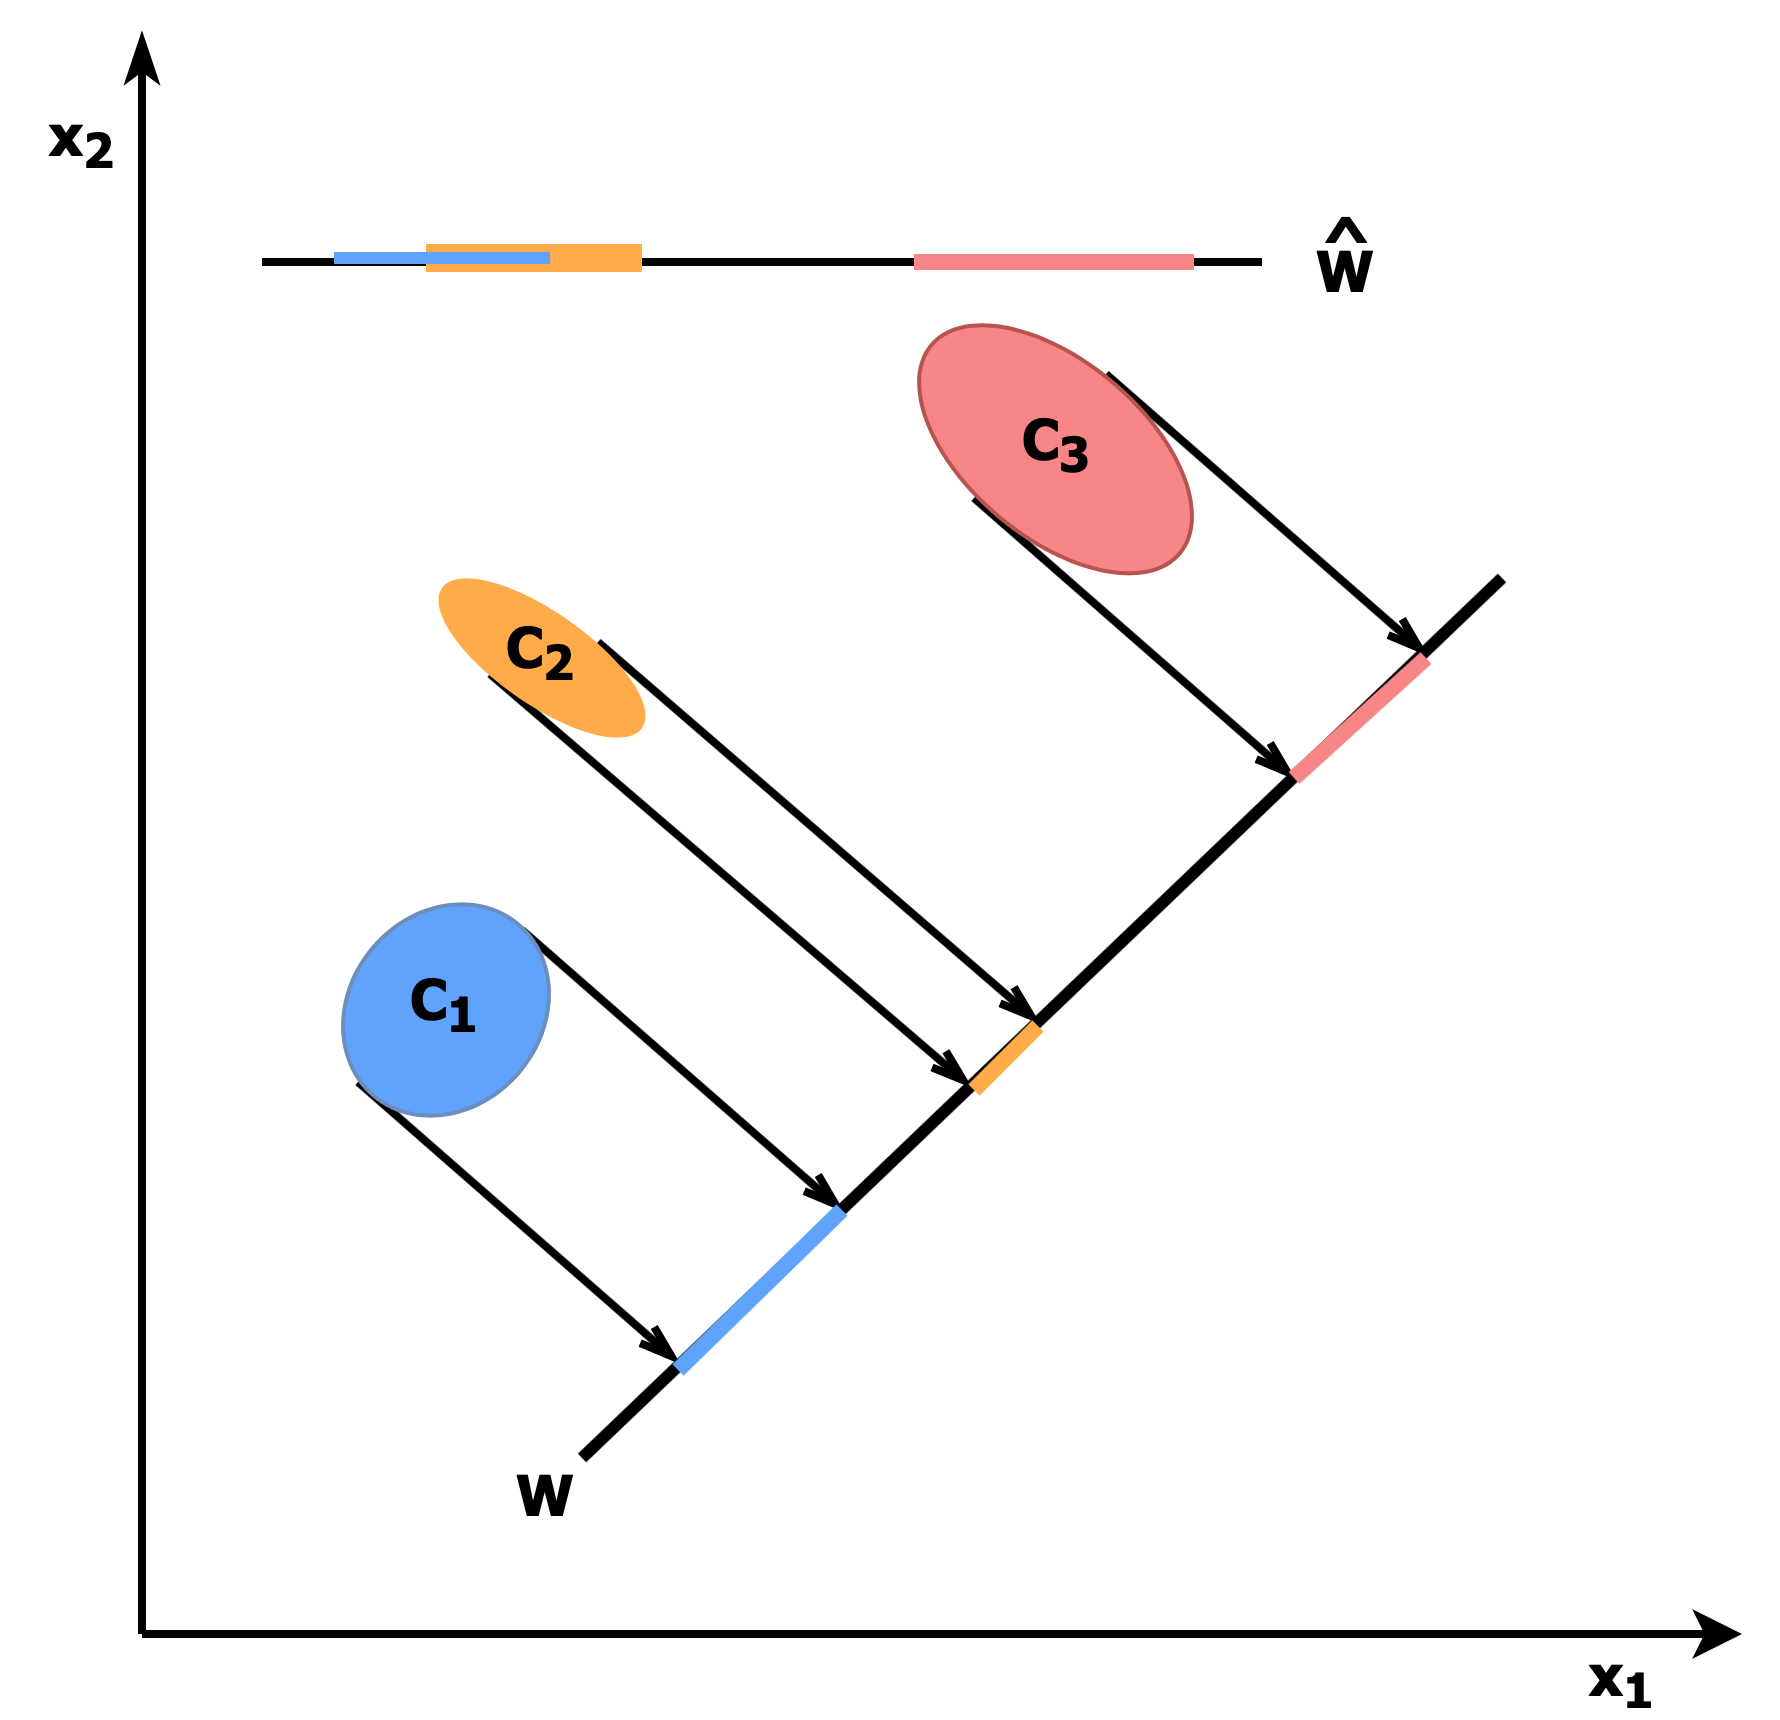
\includegraphics{graphics/dimensionality_reduction/DimensionalityReductionLDA.png}
	\caption{
		Projection of a two-dimensional feature vector to a one-dimensional feature space. 
	}
	\label{fig:dimensionalityReduction}
  \end{marginfigure}

Feature extraction using LDA \citep{Sharma2015,Huang2002} works by initially calculating the separability between the mean values of each class.

\begin{equation}
	\label{betweenClassMatrix}
	S_B = \sum^{c}_{i=1}n_{i}(\mu_i - \mu)(\mu_i - \mu)^T
	\end{equation}

This is referred to as the \textit{between-class matrix}\index{dimensionality reduction!linear discriminant analysis!between-class matrix} and is represented by equation~\ref{betweenClassMatrix}, where $c$ is the number of classes, $n_i$ is the number of samples for the $i^{th}$ class, $\mu_i$ is the mean for the $i^{th}$ class and $\mu$ is the total mean of all samples.

\begin{equation}
	\label{distanceBetweenMeanAndSampleMatrix}
	S_W = \sum^{c}_{j=1}\sum^{n_j}_{i=1}(x_{ij} - \mu_j)(x_{ij} - \mu_j)^T
	\end{equation}

Following this, the \textit{within-class matrix}\index{dimensionality reduction!linear discriminant analysis!within-class matrix} is calculated using equation~\ref{distanceBetweenMeanAndSampleMatrix}, where $c$ is the number of classes, $n_j$ is the number of samples for the $j^{th}$ class, $x_{ij}$ is the $i^{th}$ sample in the $j^{th}$ class, and $\mu_j$ is the mean for the $j^{th}$ class. This matrix indicates the distance between the mean and sample values for each class.

Finally, a \textit{transformation matrix}\index{dimensionality reduction!linear discriminant analysis!transformation matrix} $W$ which maximizes the between-class variance and minimizes the within-class variance should be constructed.

\begin{equation}
	\label{FishersCriterion}
	\arg\max_{w} \frac{W^T S_B W}{W^T S_W W}
	\end{equation}

\begin{equation}
	\label{FishersCriterion2}
	S_W W = \lambda S_B W
	\end{equation}

Fisher's criterion, shown in equation~\ref{FishersCriterion} is used to obtain the maximum ratio of the between-class matrix (denoted by $S_B$) and within class matrix (represented by $S_W$). 
By transforming the latter into equation~\ref{FishersCriterion2}, where $\lambda$ denotes the eigenvalues, eigenvectors and the corresponding eigenvalues of $W$ may be calculated.

A lower dimensional space is constructed by selecting the eigenvectors having the highest eigenvalues. 

\index{dimensionality reduction|)}